\section*{Problem 1. Benchmarks, baselines and evaluation metrics for graph
embedding on \emph{homogeneous} graphs}

\noindent
A \emph{homogeneous} graph $G=(V,E)$ carries a single node type and a single edge type:
the type-mapping functions $\phi:V\rightarrow\mathcal{A}$ and $\psi:E\rightarrow\mathcal{R}$
satisfy $|\mathcal{A}|=|\mathcal{R}|=1$. Optionally each node carries an attribute vector
$x_v\in\mathbb{R}^{d}$ and a label $y_v$. Graph embedding learns a map
$f:V\rightarrow\mathbb{R}^{k}$ with $k\ll|V|$ such that proximity in $\mathbb{R}^{k}$
reflects proximity in $G$; the embeddings are then evaluated on

\begin{itemize}[label=$\bullet$,noitemsep,topsep=2pt]
  \item \textbf{node classification} --- predict $y_v$ for held-out nodes, and
  \item \textbf{link prediction} --- score unobserved pairs $(u,v)$ so that true missing
        edges rank above non-edges.
\end{itemize}

\noindent
The heterogeneous counterpart (multiple node/edge types, metapath-based methods) is the
subject of Problem 2 and is deliberately not covered here.

\noindent
Statistics in Table~\ref{p1:tab:nodecls} were obtained by loading each graph and counting;
the OGB figures in Table~\ref{p1:tab:ogbstats} are from the official OGB documentation.
Where the literature reports conflicting values, the discrepancy is footnoted rather than
silently resolved.

%=====================================================================
\subsection*{1. Benchmark datasets}

\subsubsection*{1.1 Citation networks (the default benchmarks)}

\textbf{Cora, CiteSeer, PubMed} (Sen et al., \emph{Collective Classification in Network
Data}, AI Magazine 29(3), 2008; split protocol from Yang, Cohen \& Salakhutdinov,
\emph{Revisiting Semi-Supervised Learning with Graph Embeddings}, ICML 2016) are the three
\emph{Planetoid} citation graphs and remain the default testbed for semi-supervised node
classification. Nodes are scientific publications, an undirected edge joins two papers when
one cites the other, and the label is the paper's topic.

\textbf{Cora} collects machine-learning papers and uses \textbf{binary bag-of-words}
features.\footnote{The Cora edge count is reported inconsistently: 5{,}429 is the number of
lines in the original \texttt{cora.cites} file (which contains duplicate and
self-referential entries), 5{,}278 is the number of distinct undirected edges after
de-duplication, and 10{,}556 is the number of \emph{directed} entries stored when each
undirected edge is materialised in both directions. All three describe the same graph.}
\textbf{CiteSeer} is the sparsest of the three and has a number of isolated nodes, which is
why absolute accuracies are lowest on it. \textbf{PubMed} collects diabetes-related
biomedical abstracts and, unlike the other two, uses \textbf{real-valued TF--IDF} weights
rather than binary indicators. All three are also standard \emph{link prediction}
benchmarks: the GAE/VGAE protocol hides 5\% of edges for validation and 10\% for test,
samples an equal number of non-edges, and reports AUC and AP.

\subsubsection*{1.2 Co-authorship and co-purchase networks}

Introduced by Shchur et al.\ (\emph{Pitfalls of Graph Neural Network Evaluation}, NeurIPS
2018 Relational Representation Learning Workshop) precisely because results on the three
Planetoid graphs with a single fixed split are not statistically reliable.

\textbf{Coauthor CS} and \textbf{Coauthor Physics} come from the KDD Cup 2016 Microsoft
Academic Graph: an edge means two authors co-authored a paper, features are binary keyword
indicators over an author's papers, and the label is the author's most active field of
study. \textbf{Amazon Computers} and \textbf{Amazon Photo} are segments of the Amazon
co-purchase graph: an edge means two products are frequently bought together, features are
binary bag-of-words over product reviews, and the label is the product category. All four
are used for node classification and, being attributed and undirected, also serve as link
prediction benchmarks.

\subsubsection*{1.3 Web-page and heterophilous benchmarks (the counterexamples)}

The benchmarks above are strongly \emph{homophilous}, and a GNN that simply averages over
neighbourhoods does well on them almost by construction. The suite assembled by Pei et al.\
(\emph{Geom-GCN}, ICLR 2020) and popularised by Zhu et al.\ (\emph{Beyond Homophily in
Graph Neural Networks}, NeurIPS 2020) exists to break that assumption.

\textbf{WebKB} (\textbf{Cornell}, \textbf{Texas}, \textbf{Wisconsin}) are university web
pages linked by hyperlinks, with binary bag-of-words features and 5 page classes
(\emph{student, project, course, staff, faculty}); they are very small and very
heterophilous, so variance across splits is large and results must be averaged over the 10
standard splits. \textbf{Actor} is the actor-only induced subgraph of a
film--director--actor--writer network, where an edge means two actors are co-mentioned on
the same Wikipedia page. \textbf{Chameleon} and \textbf{Squirrel} are Wikipedia page--page
networks on those topics, with nodes binned into 5 classes by average monthly traffic. All
six are used almost exclusively for node classification.

\noindent
The quantity that separates the two groups is the \textbf{edge homophily ratio}
\begin{equation}
  h_{\mathrm{edge}}(G) \;=\; \frac{\bigl|\{(u,v)\in E : y_u = y_v\}\bigr|}{|E|},
  \label{p1:eq:homophily}
\end{equation}
which we measured directly on each graph. The values appear in the last column of
Table~\ref{p1:tab:nodecls} and range from $0.93$ (Coauthor Physics) down to $0.11$ (Texas);
Figure~\ref{p1:fig:subgraphs} illustrates the two regimes.

\noindent
\textbf{The edge set used must be stated, because two choices in it move these
numbers.}\footnote{%
\label{p1:fn:cornell}%
\emph{(i) Which edge set.} We evaluate Eq.~\eqref{p1:eq:homophily} over \emph{distinct
unordered pairs} --- precisely the set counted by the $|E|$ column of
Table~\ref{p1:tab:nodecls}, so the ratio and its denominator refer to the same object. The
six directed graphs also admit a count over the stored directed entries, which weights a
reciprocated arc twice as heavily as a one-way arc; that gives slightly different values
(e.g.\ Chameleon $0.235$ rather than $0.231$) and agrees less well with the literature.
\emph{(ii) Self-loops.} Texas and Wisconsin carry 16 each, Actor 93 and Squirrel 140, and a
self-loop trivially satisfies $y_u=y_v$, so it always counts as homophilous. Following Zhu
et al.\ we include them; excluding them would give Texas $0.06$ rather than $0.11$ and
Wisconsin $0.18$ rather than $0.21$ --- a large relative change on exactly the datasets
whose heterophily is the point. Under the stated convention our values reproduce Zhu et
al.'s published figures \emph{exactly} to two decimal places for Cora, CiteSeer, PubMed,
Texas, Wisconsin, Actor, Chameleon and Squirrel. \textbf{Cornell is the sole exception}:
Zhu et al.\ report $0.30$ and we measure $0.13$. We could not reproduce $0.30$ under any
definition we tried --- over unordered pairs $0.132$, the same excluding self-loops
$0.123$, over the stored directed entries $0.131$, or node homophily in the sense of Pei et
al.\ $0.186$ --- so we report the measured value and flag the disagreement rather than
repeating a figure we cannot reproduce.}
The ordering of the datasets is unaffected either way: the six web/Wikipedia/co-occurrence
graphs sit far below the citation, co-authorship and co-purchase graphs on any of these
definitions, which is the only claim the rest of this answer relies on.

\subsubsection*{1.4 Social and interaction networks}

These are the benchmarks of the \emph{unsupervised} embedding literature (DeepWalk, LINE,
node2vec). They are typically \textbf{feature-less} and \textbf{multi-label}, which is why
Micro-F1/Macro-F1 rather than accuracy became the standard metric in that line of work.

\textbf{BlogCatalog} is a friendship network of bloggers labelled with overlapping
interests and \textbf{Flickr} is a contact network labelled with the groups each user
joined; both are from Tang \& Liu, \emph{Relational Learning via Latent Social Dimensions},
KDD 2009. \textbf{YouTube} is a user--user social network labelled with group memberships,
from the companion paper Tang \& Liu, \emph{Scalable Learning of Collective Behavior based
on Sparse Social Dimensions}, CIKM 2009, and is the scalability stress test of that
literature. (Statistics for all three are as tabulated in the DeepWalk paper.) None has node
attributes, so structure is the only signal. \textbf{Reddit} (Hamilton, Ying \&
Leskovec, NIPS 2017) links two posts when the same user commented on both, labels each post
with its community, and is the standard \emph{inductive, large-scale} node-classification
benchmark.\footnote{We measured 57{,}307{,}946 distinct undirected edges
(114{,}615{,}892 directed entries). This reproduces the average degree of 492 stated in the
GraphSAGE paper ($2\times57{,}307{,}946/232{,}965 = 492.0$); the figure of 11.6M edges that
appears on some dataset pages refers to a sparsified copy of the graph.}

\noindent
\textbf{Warning --- three names, six graphs.} \emph{BlogCatalog}, \emph{Flickr} and
\emph{PPI} each denote two genuinely different graphs in this literature, and numbers are
frequently mixed up between them. The feature-less multi-label versions above are the ones
used by DeepWalk/node2vec; the attributed versions (BlogCatalog with 5{,}196 nodes /
171{,}743 edges / 8{,}189 features / 6 classes; the GraphSAINT Flickr with 89{,}250 nodes /
449{,}878 edges / 500 features / 7 classes) are the ones shipped by modern GNN libraries.
A paper's numbers are only comparable to another's if the same version is used.

\subsubsection*{1.5 Biological networks}

\textbf{PPI} (protein--protein interaction, GraphSAGE version) is \textbf{24 separate
graphs}, one per human tissue, whose node features are positional gene sets, motif gene sets
and immunological signatures, and whose \textbf{121 binary labels} are gene ontology terms.
The split is \emph{inductive across graphs} --- 20 train, 2 validate, 2 test --- so the test
graphs are never seen during training. This is the canonical test of whether a method
generalises to unseen graphs at all, which transductive methods such as DeepWalk cannot do
by construction. The \textbf{node2vec PPI} is a different graph: a single \emph{Homo
sapiens} subgraph with 3{,}890 nodes, 76{,}584 edges and 50 labels.

\subsubsection*{1.6 The Open Graph Benchmark (OGB)}

Hu et al.\ (\emph{Open Graph Benchmark: Datasets for Machine Learning on Graphs},
NeurIPS 2020) introduced OGB to fix the two standing problems with the classic benchmarks:
they are tiny, and their random splits are unrealistically easy. OGB fixes the split, fixes
the metric, and provides a shared evaluator, so numbers are comparable across papers.
Statistics are in Table~\ref{p1:tab:ogbstats}. The homogeneous members are:

\begin{itemize}[label=$\bullet$,noitemsep,topsep=2pt]
  \item \textbf{ogbn-arxiv} --- directed citation graph of CS arXiv papers, node features
        the averaged word2vec embedding of title and abstract, labels the 40 subject areas.
        \emph{Time split}: train up to 2017, validate on 2018, test from 2019.
  \item \textbf{ogbn-products} --- Amazon co-purchase graph, bag-of-words-plus-PCA features,
        47 top-level categories. \emph{Sales-rank split}: the most popular products train
        and the rest are validation/test, which is much harder than a random split.
  \item \textbf{ogbn-papers100M} --- the same construction as ogbn-arxiv at 111M nodes;
        only $\sim$1.5M are labelled (172 subject areas). The standard scalability benchmark.
  \item \textbf{ogbn-proteins} --- proteins from 8 species joined by weighted association
        edges. It carries \emph{edge} features and \emph{no} node features, and its 112
        binary function-prediction tasks are split \emph{by species} and scored by
        average ROC-AUC.
  \item \textbf{ogbl-collab} (author collaboration), \textbf{ogbl-ppa} (protein
        association), \textbf{ogbl-citation2} (paper citation) and \textbf{ogbl-ddi}
        (drug--drug interaction) are the four homogeneous \emph{link prediction} tasks.
        Each fixes its own split, metric and negative set in Table~\ref{p1:tab:ogbstats};
        ogbl-ddi is notable for having \emph{no} node features at all, so only structure
        can be used.
\end{itemize}

\subsubsection*{1.7 Split protocols --- and why they must be stated}

A result is meaningless without its split, because the same model can differ by many
accuracy points across protocols on the same graph:

\begin{itemize}[label=$\bullet$,noitemsep,topsep=2pt]
  \item \textbf{Planetoid semi-supervised split}: exactly \textbf{20 labelled nodes per
        class} for training, 500 for validation, 1{,}000 for test. This is the split on
        which the familiar Cora $\approx 81.5\%$ figure for GCN is reported.
  \item \textbf{Full-supervised / ``Geom-GCN'' split}: \textbf{60/20/20\%} of nodes per
        class, averaged over 10 random splits. Standard for the heterophilous benchmarks
        and typically 5--10 points higher than the 20-per-class numbers.
  \item \textbf{Random splits with fixed label budget} (Shchur et al.): the Planetoid
        budget but re-randomised, reported as mean $\pm$ std over $\geq$100 splits. This
        was the paper's central recommendation, since the single fixed Planetoid split
        does not support the ranking of methods usually claimed from it.
  \item \textbf{OGB splits} are fixed and non-random --- by time, by sales rank, by species,
        by experimental throughput, by protein target --- and deliberately induce
        distribution shift between train and test.
  \item \textbf{Link prediction}: edges, not nodes, are split. The message-passing graph
        must contain \emph{only} training edges, otherwise the held-out edge leaks into its
        own prediction. See Figure~\ref{p1:fig:linkpred}.
\end{itemize}

\begin{table}[htbp]
\centering
\small
\setlength{\tabcolsep}{4pt}
\caption{Homogeneous node-classification / link-prediction benchmarks.
\textbf{dir.}: \textbf{U} = the stored edge set is symmetric (undirected),
\textbf{D} = it is not (directed). $|E|$ counts \emph{distinct unordered pairs}, with
self-loops counted once; the parenthesised figure is the number of entries in the stored
edge list, which is $2|E|$ for the U rows but not for the D rows, since a directed graph
stores only the arcs that exist. $h_{\mathrm{edge}}$ is Eq.~\eqref{p1:eq:homophily}
measured on the graph, its denominator being exactly the $|E|$ of the preceding column ---
the same distinct unordered pairs, self-loops included (see the footnote; this convention
matters, and the alternatives are listed there). ``bin.'' = binary bag-of-words,
``TF--IDF''/``real'' = real-valued, ML = multi-label.
$^{\dagger}$Cornell: see footnote~\ref{p1:fn:cornell}.}
\label{p1:tab:nodecls}
\begin{tabular}{llrrrrccr}
\toprule
Family & Dataset & $|V|$ & $|E|$ & $d$ & \#cls & feat. & dir. & $h_{\mathrm{edge}}$ \\
\midrule
\multirow{3}{*}{Citation}
 & Cora              & 2{,}708  & 5{,}278 (10{,}556)   & 1{,}433 & 7  & bin.    & U & 0.81 \\
 & CiteSeer          & 3{,}327  & 4{,}552 (9{,}104)    & 3{,}703 & 6  & bin.    & U & 0.74 \\
 & PubMed            & 19{,}717 & 44{,}324 (88{,}648)  & 500     & 3  & TF--IDF & U & 0.80 \\
\midrule
\multirow{2}{*}{Co-author}
 & Coauthor CS       & 18{,}333 & 81{,}894             & 6{,}805 & 15 & bin.    & U & 0.81 \\
 & Coauthor Physics  & 34{,}493 & 247{,}962            & 8{,}415 & 5  & bin.    & U & 0.93 \\
\midrule
\multirow{2}{*}{Co-purchase}
 & Amazon Computers  & 13{,}752 & 245{,}861            & 767     & 10 & bin.    & U & 0.78 \\
 & Amazon Photo      & 7{,}650  & 119{,}081            & 745     & 8  & bin.    & U & 0.83 \\
\midrule
\multirow{5}{*}{Web / hyperlink}
 & Cornell           & 183      & 280 (298)            & 1{,}703 & 5  & bin.    & D & 0.13\rlap{$^{\dagger}$} \\
 & Texas             & 183      & 295 (325)            & 1{,}703 & 5  & bin.    & D & 0.11 \\
 & Wisconsin         & 251      & 466 (515)            & 1{,}703 & 5  & bin.    & D & 0.21 \\
 & Chameleon         & 2{,}277  & 31{,}421 (36{,}101)  & 2{,}325 & 5  & bin.    & D & 0.23 \\
 & Squirrel          & 5{,}201  & 198{,}493 (217{,}073)& 2{,}089 & 5  & bin.    & D & 0.22 \\
\cmidrule(l){2-9}
Co-occurrence
 & Actor             & 7{,}600  & 26{,}752 (30{,}019)  & 932     & 5  & bin.    & D & 0.22 \\
\midrule
\multirow{4}{*}{Social}
 & BlogCatalog       & 10{,}312 & 333{,}983            & ---     & 39 & none (ML) & U & --- \\
 & Flickr            & 80{,}513 & 5{,}899{,}882        & ---     & 195& none (ML) & U & --- \\
 & YouTube           & 1{,}138{,}499 & 2{,}990{,}443   & ---     & 47 & none (ML) & U & --- \\
 & Reddit            & 232{,}965 & 57{,}307{,}946      & 602     & 41 & real    & U & --- \\
\midrule
Biological
 & PPI (24 graphs)   & 56{,}944 & 793{,}632            & 50      & 121& real (ML) & U & --- \\
\bottomrule
\end{tabular}
\end{table}

\begin{table}[htbp]
\centering
\small
\setlength{\tabcolsep}{3.5pt}
\caption{The homogeneous Open Graph Benchmark datasets. Edge counts are as published by
OGB (undirected counts for undirected graphs).}
\label{p1:tab:ogbstats}
\begin{tabular}{llrrlll}
\toprule
Dataset & Domain & $|V|$ & $|E|$ & Node features & Split & Metric \\
\midrule
\multicolumn{7}{l}{\emph{Node classification}}\\
ogbn-arxiv      & citation     & 169{,}343      & 1{,}166{,}243        & 128 word2vec     & time       & Accuracy \\
ogbn-products   & co-purchase  & 2{,}449{,}029  & 61{,}859{,}140       & 100 BoW+PCA      & sales rank & Accuracy \\
ogbn-papers100M & citation     & 111{,}059{,}956& 1{,}615{,}685{,}872  & 128 word2vec     & time       & Accuracy \\
ogbn-proteins   & protein      & 132{,}534      & 39{,}561{,}252       & none (8-d edges) & species    & ROC-AUC \\
\midrule
\multicolumn{7}{l}{\emph{Link prediction}}\\
ogbl-collab     & co-authorship& 235{,}868      & 1{,}285{,}465        & 128 word2vec     & time       & Hits@50 \\
ogbl-ppa        & protein      & 576{,}289      & 30{,}326{,}273       & 58-d one-hot     & throughput & Hits@100 \\
ogbl-citation2  & citation     & 2{,}927{,}963  & 30{,}561{,}187       & 128 word2vec     & time       & MRR \\
ogbl-ddi        & drug--drug   & 4{,}267        & 1{,}334{,}889        & none             & protein target & Hits@20 \\
\bottomrule
\end{tabular}
\end{table}

%=====================================================================
\subsection*{2. Graph schemas of the benchmarks}

The \emph{graph schema} is the meta-template of a network: the graph over node types whose
edges are the permitted relation types. For a homogeneous graph the schema is by definition
\textbf{degenerate} --- one node type and one edge type --- so it is a single vertex with a
single self-loop:
\[
  \mathcal{T}_G \;=\; \bigl(\{A\},\ \{A \xrightarrow{\;R\;} A\}\bigr),
  \qquad |\mathcal{A}| = |\mathcal{R}| = 1 .
\]
This is the honest answer to ``draw the related graph schema'' for these benchmarks, and it
is exactly what distinguishes them from the heterogeneous datasets of Problem 2, whose
schemas have several node types and several relation types. What actually differs between
the homogeneous benchmarks is the \emph{semantics} instantiated into $A$ and $R$, so the
benchmarks are grouped into seven schema families in Figure~\ref{p1:fig:schemas}. Because a
one-node schema is visually vacuous on its own, Figure~\ref{p1:fig:subgraphs} additionally
sketches the local structure that the schema does \emph{not} capture and which nevertheless
drives model performance: the label homophily of Eq.~\eqref{p1:eq:homophily}.

\begin{figure}[htbp]
\centering
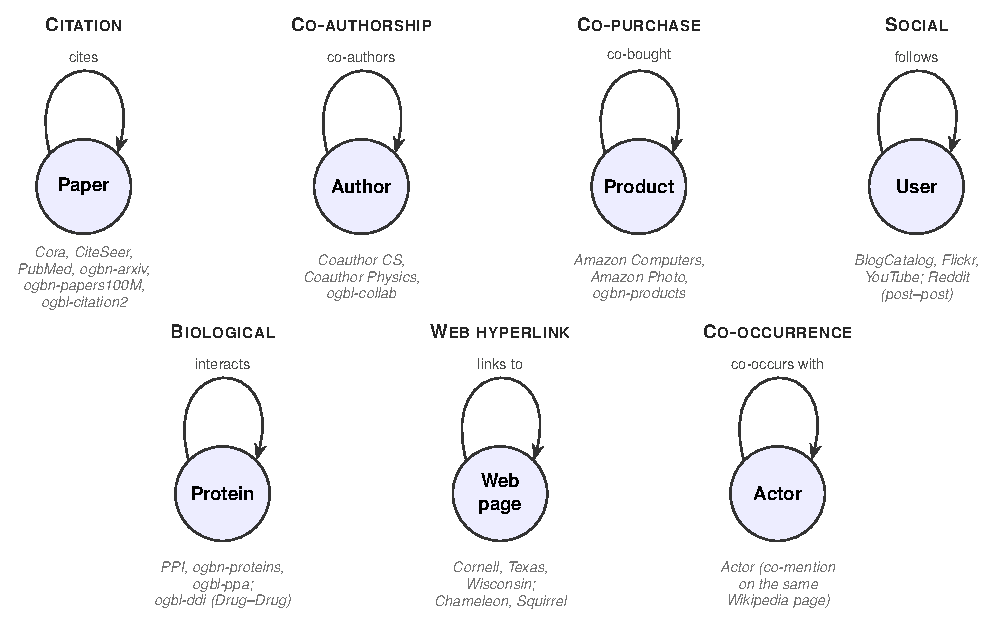
\includegraphics[width=\textwidth]{fig_p1_schema_families.pdf}
\caption{Graph schemas of the homogeneous benchmarks, grouped into seven families. Every
schema is a single node type with a single self-relation; only the interpretation of the
node and the edge changes between families.}
\label{p1:fig:schemas}
\end{figure}

\begin{figure}[htbp]
\centering
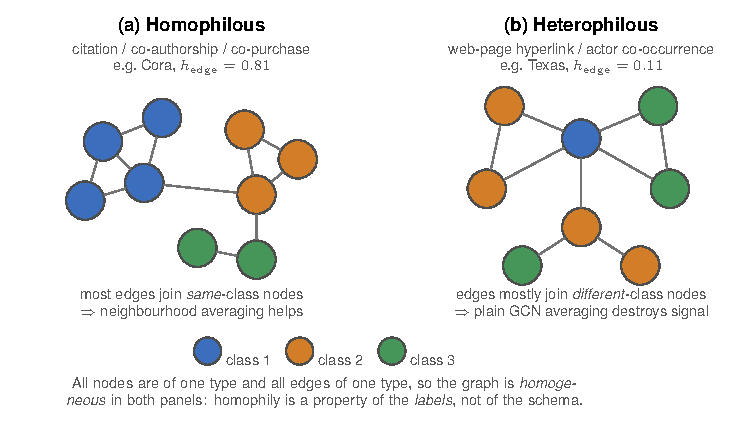
\includegraphics[width=0.78\textwidth]{fig_p1_subgraphs.pdf}
\caption{Illustrative subgraphs. Both graphs have the same (degenerate) schema; they differ
in how labels are distributed over edges. The measured $h_{\mathrm{edge}}$ values are those
of Table~\ref{p1:tab:nodecls}.}
\label{p1:fig:subgraphs}
\end{figure}

%=====================================================================
\subsection*{3. Baselines}

\subsubsection*{3.1 Matrix factorisation and spectral methods}

\begin{itemize}[label=$\bullet$,leftmargin=1.3em]
  \item \textbf{Laplacian Eigenmaps} --- Belkin \& Niyogi, \emph{Laplacian Eigenmaps and
        Spectral Techniques for Embedding and Clustering}, NIPS 2001; expanded as
        \emph{Laplacian Eigenmaps for Dimensionality Reduction and Data Representation},
        \emph{Neural Computation} 15(6):1373--1396, 2003 (the canonical citation).
        Embeds nodes by the eigenvectors of the graph Laplacian $L = D - A$ belonging to
        the smallest non-zero eigenvalues, i.e.\ it minimises
        $\sum_{(u,v)\in E} w_{uv}\lVert f(u)-f(v)\rVert^2$ subject to an orthogonality
        constraint ruling out the trivial solution. The ancestor of essentially every
        proximity-preserving embedding; spectral clustering is the same computation.
  \item \textbf{GraRep} --- Cao, Lu \& Xu, \emph{GraRep: Learning Graph Representations with
        Global Structural Information}, CIKM 2015.
        Observes that first-order proximity is not enough, and factorises the
        \emph{$k$-step} transition matrices $P^1,\dots,P^K$ (via SVD of their log-transformed
        positive entries) separately, concatenating the $K$ resulting embeddings. This
        captures $k$-hop structure explicitly, at the cost of dense $|V|\times|V|$ powers.
  \item \textbf{HOPE} --- Ou, Cui, Pei, Zhang \& Zhu, \emph{Asymmetric Transitivity
        Preserving Graph Embedding}, KDD 2016.
        Targets \emph{directed} graphs, where proximity is asymmetric. It learns two
        vectors per node (source and target) and factorises a high-order proximity matrix
        --- Katz, Rooted PageRank, Common Neighbors or Adamic--Adar --- which it shows can
        be written in a sparse form $S = M_g^{-1}M_\ell$ admitting a generalised SVD, so the
        cost is linear in $|E|$.
  \item \textbf{NetMF} --- Qiu, Dong, Ma, Li, Wang \& Tang, \emph{Network Embedding as
        Matrix Factorization: Unifying DeepWalk, LINE, PTE, and node2vec}, WSDM 2018.
        Proves that the skip-gram-with-negative-sampling objectives of DeepWalk, LINE, PTE
        and node2vec all implicitly factorise a closed-form matrix, for DeepWalk
        $\log\bigl(\tfrac{\mathrm{vol}(G)}{bT}(\sum_{r=1}^{T}P^r)D^{-1}\bigr)$. Factorising
        that matrix directly gives better embeddings than running the sampler, and the
        paper is the standard theoretical bridge between the random-walk and
        factorisation families.
\end{itemize}

\subsubsection*{3.2 Random-walk / skip-gram methods}

\begin{itemize}[label=$\bullet$,leftmargin=1.3em]
  \item \textbf{DeepWalk} --- Perozzi, Al-Rfou \& Skiena, \emph{DeepWalk: Online Learning of
        Social Representations}, KDD 2014.
        The paper that started the field. It samples uniform random walks from each node,
        treats each walk as a ``sentence'' and each node as a ``word'', and runs
        word2vec/skip-gram with hierarchical softmax over them. Nodes appearing in similar
        walk contexts receive similar vectors. It requires no node attributes and is
        trivially parallel, but is transductive: unseen nodes have no embedding.
  \item \textbf{LINE} --- Tang, Qu, Wang, Zhang, Yan \& Mei, \emph{LINE: Large-scale
        Information Network Embedding}, WWW 2015.
        Dispenses with walks and optimises two explicit objectives: \emph{first-order}
        proximity (observed edges, $p_1(u,v)=\sigma(f(u)^{\!\top}f(v))$) and
        \emph{second-order} proximity (shared neighbourhoods, a context embedding per node),
        each trained by negative sampling with edge-sampling to handle weights. The two
        embeddings are concatenated. It scales to millions of nodes and is the standard
        ``no-walk'' baseline.
  \item \textbf{node2vec} --- Grover \& Leskovec, \emph{node2vec: Scalable Feature Learning
        for Networks}, KDD 2016.
        Generalises DeepWalk by biasing the walk with return parameter $p$ and in-out
        parameter $q$, interpolating between breadth-first search (which captures
        \emph{structural equivalence}) and depth-first search (which captures
        \emph{homophily}). Tuning $(p,q)$ per dataset is what buys its consistent gain over
        DeepWalk. It also defines the standard Hadamard/L1/L2 binary operators for turning
        node embeddings into edge features for link prediction.
  \item \textbf{struc2vec} --- Ribeiro, Savarese \& Figueiredo, \emph{struc2vec: Learning
        Node Representations from Structural Identity}, KDD 2017.
        Argues that nodes with similar \emph{roles} should embed together even if they are
        far apart in the graph --- something no proximity-based method can do. It builds a
        multilayer context graph whose layer-$k$ edge weights compare the ordered degree
        sequences of $k$-hop neighbourhoods, then runs skip-gram on walks over that
        auxiliary graph.
\end{itemize}

\subsubsection*{3.3 Autoencoder methods}

\begin{itemize}[label=$\bullet$,leftmargin=1.3em]
  \item \textbf{SDNE} --- Wang, Cui \& Zhu, \emph{Structural Deep Network Embedding},
        KDD 2016.
        A deep autoencoder whose input is a node's adjacency row. It combines a
        reconstruction loss on that row (second-order proximity), re-weighted so that the
        many zeros do not dominate the few ones, with a Laplacian-eigenmaps-style penalty
        tying connected nodes together (first-order proximity). The first non-linear
        (deep) network embedding method.
  \item \textbf{GAE / VGAE} --- Kipf \& Welling, \emph{Variational Graph Auto-Encoders},
        NIPS 2016 Bayesian Deep Learning Workshop.
        Uses a two-layer GCN as the encoder, $Z=\mathrm{GCN}(X,A)$, and a simple inner-product
        decoder $\hat{A}=\sigma(ZZ^{\!\top})$, trained by reconstruction cross-entropy; the
        variational version places a Gaussian prior on $Z$ and adds a KL term. It is the
        default \emph{unsupervised} baseline for link prediction on Cora/CiteSeer/PubMed.
\end{itemize}

\subsubsection*{3.4 Graph neural networks (message passing)}

All of these compute $h_v^{(l+1)} = \mathrm{UPDATE}\bigl(h_v^{(l)},
\mathrm{AGGREGATE}(\{h_u^{(l)}: u\in\mathcal{N}(v)\})\bigr)$ and differ in the two functions.

\begin{itemize}[label=$\bullet$,leftmargin=1.3em]
  \item \textbf{GCN} --- Kipf \& Welling, \emph{Semi-Supervised Classification with Graph
        Convolutional Networks}, ICLR 2017.
        A first-order approximation of a Chebyshev spectral filter, giving the layer
        $H^{(l+1)} = \sigma\bigl(\tilde{D}^{-1/2}\tilde{A}\tilde{D}^{-1/2}H^{(l)}W^{(l)}\bigr)$
        with $\tilde{A}=A+I$. It is a symmetrically-normalised neighbourhood average
        followed by a linear map; two layers is the standard configuration. The single most
        reported baseline in the field.
  \item \textbf{GraphSAGE} --- Hamilton, Ying \& Leskovec, \emph{Inductive Representation
        Learning on Large Graphs}, NIPS 2017.
        Makes GNNs \emph{inductive} and scalable: instead of using the full adjacency it
        samples a fixed number of neighbours per hop and learns an aggregator (mean, LSTM
        or max-pool) plus a concatenation with the node's own previous representation.
        Because the aggregator is shared, embeddings can be produced for nodes --- and
        graphs --- never seen in training. Introduced the Reddit and PPI benchmarks.
  \item \textbf{GAT} --- Veli\v{c}kovi\'{c}, Cucurull, Casanova, Romero, Li\`{o} \& Bengio,
        \emph{Graph Attention Networks}, ICLR 2018.
        Replaces the fixed normalisation coefficient $1/\sqrt{d_ud_v}$ with a learned
        attention weight $\alpha_{uv}=\mathrm{softmax}_u\bigl(\mathrm{LeakyReLU}(a^{\!\top}
        [Wh_v \Vert Wh_u])\bigr)$, so a node can weight its neighbours unequally. Multi-head
        attention stabilises training. No spectral decomposition and no knowledge of the
        full graph is required, so it too is inductive.
  \item \textbf{JK-Net} --- Xu, Li, Tian, Sonobe, Kawarabayashi \& Jegelka,
        \emph{Representation Learning on Graphs with Jumping Knowledge Networks}, ICML 2018.
        Observes that the right neighbourhood radius differs per node (hub vs.\ periphery),
        and lets the final representation ``jump'' by combining \emph{all} intermediate
        layers $h^{(1)},\dots,h^{(L)}$ via concatenation, max-pooling or an LSTM attention,
        rather than using only the last. A standard remedy for over-smoothing.
  \item \textbf{GIN} --- Xu, Hu, Leskovec \& Jegelka, \emph{How Powerful are Graph Neural
        Networks?}, ICLR 2019.
        Analyses message passing through the Weisfeiler--Lehman test and shows that mean and
        max aggregation lose information; a \emph{sum} aggregator with an MLP update,
        $h_v^{(l+1)}=\mathrm{MLP}\bigl((1+\epsilon)h_v^{(l)}+\sum_{u\in\mathcal{N}(v)}h_u^{(l)}\bigr)$,
        is maximally expressive, i.e.\ as strong as 1-WL. The reference point for all
        expressive-power arguments.
  \item \textbf{SGC} --- Wu, Souza, Zhang, Fifty, Yu \& Weinberger, \emph{Simplifying Graph
        Convolutional Networks}, ICML 2019.
        Removes every non-linearity from a $K$-layer GCN, collapsing it to
        $\hat{Y}=\mathrm{softmax}(S^K X W)$ with $S=\tilde{D}^{-1/2}\tilde{A}\tilde{D}^{-1/2}$.
        Since $S^KX$ is a fixed pre-computation, training is plain logistic regression ---
        orders of magnitude faster, and on the homophilous citation benchmarks essentially
        as accurate. An important sanity baseline: it measures how much the non-linearity
        was really contributing.
  \item \textbf{APPNP} --- Gasteiger (formerly Klicpera), Bojchevski \& G\"unnemann,
        \emph{Predict then Propagate: Graph Neural Networks meet Personalized PageRank},
        ICLR 2019.
        Decouples prediction from propagation: an MLP produces per-node predictions $H$,
        which are then diffused by a truncated personalized-PageRank iteration
        $Z^{(k+1)} = (1-\alpha)\hat{A}Z^{(k)} + \alpha H$. The teleport term $\alpha$ keeps
        the node's own signal alive, so a large propagation radius is possible without
        over-smoothing and without extra parameters.
  \item \textbf{GCNII} --- Chen, Wei, Huang, Ding \& Li, \emph{Simple and Deep Graph
        Convolutional Networks}, ICML 2020.
        Makes genuinely deep GCNs (32--64 layers) work using two ingredients: an
        \emph{initial residual} connection to $H^{(0)}$ (the APPNP teleport idea) and
        \emph{identity mapping} of the weight matrix, $(1-\beta_l)I + \beta_l W^{(l)}$.
        Proves the result still expresses a polynomial filter of arbitrary order and so
        does not collapse to over-smoothing.
  \item \textbf{SEAL} --- Zhang \& Chen, \emph{Link Prediction Based on Graph Neural
        Networks}, NeurIPS 2018.
        Reframes link prediction as \emph{subgraph classification}: for a candidate pair
        $(u,v)$ it extracts the $h$-hop enclosing subgraph, applies a Double-Radius Node
        Labeling that encodes each node's distance to both $u$ and $v$, and classifies the
        labelled subgraph with a GNN. The $\gamma$-decaying theory in the paper shows such
        a GNN can learn any of the classical heuristics below rather than assuming one.
        The strongest general-purpose link-prediction baseline.
  \item \textbf{NBFNet} --- Zhu, Zhang, Xhonneux \& Tang, \emph{Neural Bellman-Ford
        Networks: A General Graph Neural Network Framework for Link Prediction},
        NeurIPS 2021.
        Generalises the Bellman--Ford path formulation by replacing $(\min,+)$ with learned
        \textsc{Indicator}, \textsc{Message} and \textsc{Aggregate} operators, so the score
        for $(u,v)$ is a learned sum over all paths from $u$ to $v$. Inductive (it depends
        on structure relative to $u$, not on node identity) and applies to homogeneous
        graphs and knowledge graphs alike.
\end{itemize}

\subsubsection*{3.5 Self-supervised and contrastive methods}

\begin{itemize}[label=$\bullet$,leftmargin=1.3em]
  \item \textbf{DGI} --- Veli\v{c}kovi\'{c}, Fedus, Hamilton, Li\`{o}, Bengio \& Hjelm,
        \emph{Deep Graph Infomax}, ICLR 2019.
        Maximises the mutual information between patch representations $h_v$ and a global
        summary $s$ of the graph, using a discriminator trained to tell real
        $(h_v,s)$ pairs from corrupted ones (the corruption shuffles the node features).
        Needs no random walks and no labels, and was the first unsupervised method to match
        supervised GCN on the citation benchmarks.
  \item \textbf{GRACE} --- Zhu, Xu, Yu, Liu, Wu \& Wang, \emph{Deep Graph Contrastive
        Representation Learning}, ICML 2020 Workshop on Graph Representation Learning and
        Beyond.
        A node-level SimCLR analogue: generate two views by removing edges and masking
        features, then maximise agreement between the two representations of the same node
        against all other nodes as negatives (InfoNCE). Contrasts at node rather than
        graph-summary level, which DGI does not.
  \item \textbf{GraphCL} --- You, Chen, Sui, Chen, Wang \& Shen, \emph{Graph Contrastive
        Learning with Augmentations}, NeurIPS 2020.
        Systematically studies four graph augmentations --- node dropping, edge
        perturbation, attribute masking and subgraph sampling --- and shows which
        combinations help on which domain. Mostly graph-level, but its augmentation study
        is the reference for the whole contrastive family.
  \item \textbf{BGRL} --- Thakoor, Tallec, Azar, Azabou, Dyer, Munos, Veli\v{c}kovi\'{c} \&
        Valko, \emph{Large-Scale Representation Learning on Graphs via Bootstrapping},
        ICLR 2022.
        Removes negative samples altogether using a BYOL-style online/target encoder pair
        with a stop-gradient, cutting memory from quadratic to linear in the number of
        nodes. This is what makes self-supervised learning feasible at OGB scale.
\end{itemize}

\subsubsection*{3.6 Non-learned link-prediction heuristics}

Every link-prediction paper reports these; they are strong, free, and a learned method that
does not beat them is not worth its compute. The framing is due to Liben-Nowell \& Kleinberg
(\emph{The Link Prediction Problem for Social Networks}, CIKM 2003; journal version JASIST
58(7), 2007). Let $\Gamma(u)$ be the neighbour set of $u$ and $A$ the adjacency matrix.

\begin{center}
\footnotesize
\setlength{\tabcolsep}{4pt}
\renewcommand{\arraystretch}{1.35}
\begin{tabular}{@{}>{\raggedright\arraybackslash}p{2.35cm}
                  >{\raggedright\arraybackslash}p{5.5cm}
                  >{\raggedright\arraybackslash}p{6.3cm}@{}}
\toprule
Heuristic & Score $s(u,v)$ & Reference / note \\
\midrule
Common Neighbors & $|\Gamma(u)\cap\Gamma(v)|$ &
  Liben-Nowell \& Kleinberg, CIKM 2003 \\
Jaccard & $|\Gamma(u)\cap\Gamma(v)| \,/\, |\Gamma(u)\cup\Gamma(v)|$ &
  normalises CN by degree \\
Adamic--Adar & $\textstyle\sum_{w\in\Gamma(u)\cap\Gamma(v)} 1/\log|\Gamma(w)|$ &
  Adamic \& Adar, \emph{Friends and Neighbors on the Web}, Social Networks 25(3), 2003 \\
Resource Allocation & $\textstyle\sum_{w\in\Gamma(u)\cap\Gamma(v)} 1/|\Gamma(w)|$ &
  Zhou, L\"u \& Zhang, \emph{Eur.\ Phys.\ J.\ B} 71(4), 2009; penalises hubs harder than AA \\
Preferential Attachment & $|\Gamma(u)|\cdot|\Gamma(v)|$ &
  Barab\'asi \& Albert, \emph{Science} 286, 1999 \\
Katz & $\textstyle\sum_{\ell\geq1}\beta^{\ell}\bigl|\mathrm{paths}^{\langle\ell\rangle}_{u,v}\bigr|
        = \bigl((I-\beta A)^{-1}-I\bigr)_{uv}$ &
  Katz, \emph{Psychometrika} 18(1), 1953; global, needs $\beta<1/\lambda_{\max}$ \\
Personalized PageRank & stationary probability at $v$ of a random walk from $u$ with restart &
  Jeh \& Widom, \emph{Scaling Personalized Web Search}, WWW 2003; PageRank itself: Page, Brin, Motwani \& Winograd, Stanford InfoLab TR, 1999 \\
SimRank & $\dfrac{\gamma}{|\Gamma(u)||\Gamma(v)|}
           \textstyle\sum_{a\in\Gamma(u)}\sum_{b\in\Gamma(v)} s(a,b)$ &
  Jeh \& Widom, KDD 2002; ``similar if referenced by similar nodes'' \\
\bottomrule
\end{tabular}
\end{center}

\noindent
The first five are \emph{local} (2-hop) and therefore cheap but blind to long-range
structure; Katz, PPR and SimRank are \emph{global} and stronger but cost a matrix inverse or
an iterative solve. On ogbl-ddi and ogbl-ppa, Common Neighbors and Adamic--Adar remain
competitive with many GNNs, which is the usual argument for reporting them.

%=====================================================================
\subsection*{4. Evaluation metrics}

\subsubsection*{4.1 Node classification}

Let $C$ be the number of classes and $\mathrm{TP}_c,\mathrm{FP}_c,\mathrm{FN}_c$ the
per-class counts.

\begin{itemize}[label=$\bullet$,leftmargin=1.3em]
  \item \textbf{Accuracy} $=\frac{1}{|V_{\text{test}}|}\sum_v \mathbf{1}[\hat{y}_v = y_v]$.
        The default for single-label benchmarks (Planetoid, OGB node tasks). Misleading
        under class imbalance.
  \item \textbf{Precision / Recall / F1} per class:
        $P_c = \frac{\mathrm{TP}_c}{\mathrm{TP}_c+\mathrm{FP}_c}$,
        $R_c = \frac{\mathrm{TP}_c}{\mathrm{TP}_c+\mathrm{FN}_c}$,
        $F1_c = \frac{2P_cR_c}{P_c+R_c}$.
  \item \textbf{Micro-F1} --- pool the confusion matrix over all classes first, then compute
        one F1:
        \begin{equation}
          \text{Micro-F1} \;=\; \frac{2\sum_c \mathrm{TP}_c}
            {2\sum_c \mathrm{TP}_c + \sum_c \mathrm{FP}_c + \sum_c \mathrm{FN}_c}.
          \label{p1:eq:microf1}
        \end{equation}
        In single-label multi-class classification every error is simultaneously one FP and
        one FN, so \textbf{Micro-F1 $=$ Accuracy}. It is dominated by the frequent classes.
  \item \textbf{Macro-F1} --- the \emph{unweighted} mean of the per-class F1 scores:
        \begin{equation}
          \text{Macro-F1} \;=\; \frac{1}{C}\sum_{c=1}^{C} F1_c .
          \label{p1:eq:macrof1}
        \end{equation}
        Because every class contributes equally regardless of size, a model that ignores a
        rare class is punished. \textbf{This is why Macro-F1 matters}: on BlogCatalog or
        Flickr, where label frequencies span orders of magnitude, a model can score well on
        Micro-F1 while never predicting most of the 39 (resp.\ 195) labels --- the gap
        between the two numbers is the diagnostic, and reporting only Micro-F1 hides it.
  \item \textbf{ROC-AUC}, computed one-vs-rest and averaged over classes for multi-class
        problems, and averaged over tasks for multi-label problems (this is the ogbn-proteins
        metric). It is threshold-free, so it measures ranking quality rather than the
        quality of a particular decision threshold.
  \item \textbf{Reporting convention.} A single number is not a result. The convention is
        \textbf{mean $\pm$ standard deviation over 10 (OGB, fixed split, 10 seeds) or 100
        (Shchur et al., random splits) runs}, since the spread across splits on the small
        benchmarks routinely exceeds the differences between published methods.
  \item \textbf{Protocol for unsupervised embeddings.} DeepWalk/LINE/node2vec/DGI are
        evaluated by the \emph{linear-probe} protocol: learn the embedding with no labels,
        \textbf{freeze} it, train a one-vs-rest $\ell_2$-regularised logistic regression on
        the embeddings of a fraction $\rho$ of nodes, and report Micro-F1 and Macro-F1 on
        the rest. Results are given as a curve over training ratios
        $\rho\in\{10\%,\dots,90\%\}$ (BlogCatalog) or $\{1\%,\dots,10\%\}$ (Flickr, YouTube).
        Freezing is essential --- fine-tuning the encoder would measure something else.
\end{itemize}

\subsubsection*{4.2 Link prediction}

Link prediction is extremely class-imbalanced (a graph with $|V|$ nodes has
$\binom{|V|}{2}\!-\!|E|$ non-edges), so the metric choice matters far more than for node
classification. Positives are held-out edges; negatives are sampled node pairs that are not
edges (Figure~\ref{p1:fig:linkpred}).

\begin{itemize}[label=$\bullet$,leftmargin=1.3em]
  \item \textbf{AUC-ROC} --- the probability that a random positive outranks a random
        negative. Standard in the GAE/VGAE protocol with a $1\!:\!1$ positive:negative
        ratio.
  \item \textbf{Average Precision (AP / AUPRC)} ---
        \begin{equation}
          \mathrm{AP} \;=\; \sum_{k} \bigl(R_k - R_{k-1}\bigr)\,P_k ,
          \label{p1:eq:ap}
        \end{equation}
        with $P_k,R_k$ the precision and recall at threshold rank $k$. Unlike AUC it does
        not credit a model for correctly ranking the vast easy majority of negatives.
  \item \textbf{Precision@K / Recall@K} --- the fraction of the top-$K$ predicted pairs that
        are true edges, and the fraction of true edges recovered in the top $K$.
  \item \textbf{Hits@K} --- the fraction of positive edges ranked in the top $K$ against the
        sampled negatives:
        \begin{equation}
          \mathrm{Hits@}K \;=\; \frac{1}{|E_{\text{test}}|}
            \sum_{e\in E_{\text{test}}} \mathbf{1}\bigl[\mathrm{rank}(e) \leq K\bigr].
          \label{p1:eq:hits}
        \end{equation}
        OGB fixes $K$ per dataset so that numbers are comparable: \textbf{Hits@50} for
        ogbl-collab (against 100{,}000 shared negatives), \textbf{Hits@20} for ogbl-ddi,
        \textbf{Hits@100} for ogbl-ppa (against 3{,}000{,}000 negatives).
  \item \textbf{MRR} --- for each query (in ogbl-citation2, each source paper, ranked against
        1{,}000 sampled negative references),
        \begin{equation}
          \mathrm{MRR} \;=\; \frac{1}{|Q|}\sum_{q\in Q} \frac{1}{\mathrm{rank}_q},
          \label{p1:eq:mrr}
        \end{equation}
        where $\mathrm{rank}_q$ is the position of the first true item for query $q$.
        Rewards getting the answer at the very top far more than at position 10.
  \item \textbf{NDCG@K} --- with $\mathrm{rel}_i$ the relevance of the item at rank $i$,
        \begin{equation}
          \mathrm{DCG@}K=\sum_{i=1}^{K}\frac{2^{\mathrm{rel}_i}-1}{\log_2(i+1)},
          \qquad
          \mathrm{NDCG@}K=\frac{\mathrm{DCG@}K}{\mathrm{IDCG@}K},
          \label{p1:eq:ndcg}
        \end{equation}
        $\mathrm{IDCG@}K$ being the DCG of the ideal ordering. Used when a node has many
        true links of differing importance (recommendation-style evaluation).
\end{itemize}

\paragraph{Negative sampling, and why AUC is optimistic.}
The negatives define the metric. Three conventions are in use: (i) \emph{$1\!:\!1$ random
negatives} (the GAE protocol), (ii) \emph{a shared fixed negative set} for all positives
(ogbl-collab, ogbl-ddi, ogbl-ppa), and (iii) \emph{per-query negatives}
(ogbl-citation2: 1{,}000 previously-published papers per source node). Real graphs are
sparse, so a uniformly sampled pair is almost always a pair of distant, low-degree nodes
that any model rejects trivially. AUC averages over all such pairs and therefore saturates
near $1.0$ and stops discriminating between methods --- this is precisely why OGB abandoned
it in favour of Hits@K and MRR, which only reward ranking the positive above the
\emph{hardest} sampled negatives. AP is likewise more informative than AUC because it
weights the high-precision region where the model actually operates. A corollary is that
Hits@K numbers are \emph{only} comparable when the negative set is identical, which is the
reason OGB ships a fixed evaluator.

\begin{figure}[htbp]
\centering
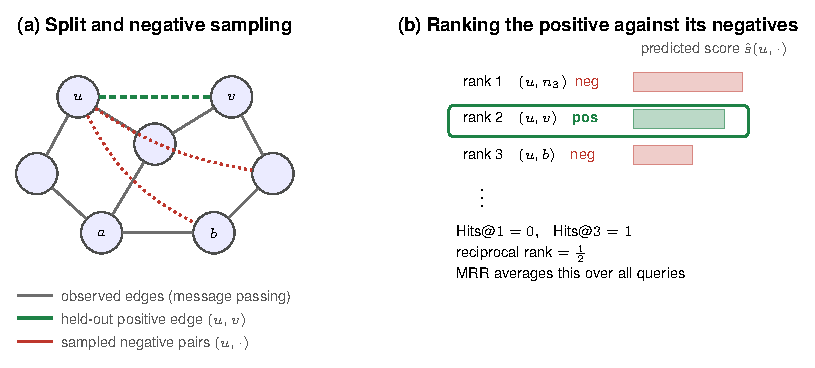
\includegraphics[width=0.84\textwidth]{fig_p1_linkpred.pdf}
\caption{The link-prediction evaluation protocol. The held-out positive edge must be removed
from the message-passing graph, and is scored against a sampled set of negatives; Hits@K and
MRR are read off the resulting ranking.}
\label{p1:fig:linkpred}
\end{figure}

\subsubsection*{4.3 Which metric is reported on which dataset}

\begin{table}[htbp]
\centering
\small
\caption{Dataset $\rightarrow$ task $\rightarrow$ metric normally reported.}
\label{p1:tab:metrics}
\setlength{\tabcolsep}{4pt}
\begin{tabular}{@{}>{\raggedright\arraybackslash}p{4.1cm}
                  >{\raggedright\arraybackslash}p{3.6cm}
                  >{\raggedright\arraybackslash}p{6.9cm}@{}}
\toprule
Dataset & Task & Metric normally reported \\
\midrule
Cora / CiteSeer / PubMed & node classification & Accuracy ($=$ Micro-F1), mean $\pm$ std over 10--100 splits \\
Cora / CiteSeer / PubMed & link prediction     & AUC-ROC and AP (GAE protocol, 85/5/10 edge split) \\
Coauthor CS / Physics    & node classification & Accuracy, mean $\pm$ std over 100 random splits \\
Amazon Computers / Photo & node classification & Accuracy, mean $\pm$ std over 100 random splits \\
WebKB, Actor, Chameleon, Squirrel & node classification & Accuracy over the 10 fixed 60/20/20 splits \\
BlogCatalog / Flickr / YouTube & node classification, multi-label & Micro-F1 and Macro-F1 vs.\ training ratio \\
PPI (24 graphs) & inductive node classification, multi-label & Micro-F1 \\
Reddit & inductive node classification & Micro-F1 ($=$ Accuracy) \\
ogbn-arxiv / products / papers100M & node classification & Accuracy (fixed OGB split) \\
ogbn-proteins & node classification, 112 tasks & ROC-AUC averaged over tasks \\
ogbl-collab & link prediction & Hits@50 (100{,}000 shared negatives) \\
ogbl-ddi & link prediction & Hits@20 ($\sim$100{,}000 shared negatives) \\
ogbl-ppa & link prediction & Hits@100 (3{,}000{,}000 shared negatives) \\
ogbl-citation2 & link prediction & MRR (1{,}000 negatives per source node) \\
\bottomrule
\end{tabular}
\end{table}

%=====================================================================
\subsection*{5. Summary}

For homogeneous graphs the schema is degenerate --- one node type, one edge type
(Figure~\ref{p1:fig:schemas}) --- so what distinguishes the benchmarks is scale, feature
type, and above all label homophily (Eq.~\eqref{p1:eq:homophily}). The suite has moved in
three waves: the small homophilous citation graphs with a fixed 20-per-class split, the
re-splittable co-authorship/co-purchase graphs and the heterophilous WebKB/Wikipedia graphs
introduced to expose the homophily assumption, and finally OGB, with realistic non-random
splits and a shared evaluator at a scale where sampling-based training is mandatory. On
metrics, the two points that matter most are that Micro-F1 equals accuracy in the
single-label case while Macro-F1 is what exposes neglected rare classes, and that on sparse
graphs AUC is optimistic, so ranking metrics against a \emph{fixed} negative set (Hits@K,
MRR) are what make link-prediction results comparable.
